\documentclass[conference]{IEEEtran}
\IEEEoverridecommandlockouts

\usepackage{cite}
\usepackage{amsmath,amssymb,amsfonts}
\usepackage{algorithm}
\usepackage{algpseudocode}
\usepackage{graphicx}
\usepackage{textcomp}
\usepackage{xcolor}
\usepackage{array}

\def\BibTeX{{\rm B\kern-.05em{\sc i\kern-.025em b}\kern-.08em
    T\kern-.1667em\lower.7ex\hbox{E}\kern-.125em X}}

\begin{document}

\title{EchoMind: A Voice-Based AI Companion that Detects Reasoning Blind Spots Using Multimodal Emotion Fusion and Gentle, Adaptive Feedback}

% ------------------------------------------------------------------
% AUTHORS -- 2 authors per row, e-mail on a single line.
% Change e-mails / names here only.
% ------------------------------------------------------------------
\newcommand{\authorbox}[2]{%
  \begin{minipage}[t]{0.46\textwidth}
    \centering
    {\fontsize{11}{13}\selectfont #1}\\
    #2\\
    \textit{VIT-AP University}, Amaravati, India
  \end{minipage}}

\author{%
\parbox{\textwidth}{\centering
\authorbox{A. Sri Charan}{charan.23bce7702@vitapstudent.ac.in}%
\hfill
\authorbox{M. Sravya}{sravya.24bca7630@vitapstudent.ac.in}%
\\[1.5ex]
\authorbox{M. Sai Shivani}{shivani.24bca7713@vitapstudent.ac.in}%
\hfill
\authorbox{Mahak Agarwal}{mahak.24bca7783@vitapstudent.ac.in}%
}}

\maketitle

\begin{abstract}
When people speak out their decisions, hidden cognitive distortions and reasoning blind spots---such as logical jumps, generalizations, or emotional reasoning---often sabotage decision quality. Existing conversational AI assistants focus on empathetic validation or static text-based Socratic dialogue, but fail to evaluate the real-time logical validity of the spoken argument or adjust feedback strength according to the emotional distress of the speaker expressed through voice. To tackle this problem, we propose EchoMind, a voice-based deep learning companion designed to detect reasoning blind spots during problem-solving conversations and provide distress-dependent, reflective interventions. EchoMind employs an innovative six-step multimodal architecture consisting of: mono 16~kHz audio input; dual-modality emotion extraction based on acoustic prosody and text sentiment using TF-IDF; confidence-weighted feature fusion; an eight-class cognitive distortion classifier enhanced by regular expressions and Google Gemini LLM validation; a distress-dependent intervention policy; and a reflection loop with memory persistence. We test our proposed system on an integrated browser prototype across different dataset partitions. Finally, we discuss the architecture details, algorithmic logic, and baselines of EchoMind, and describe how this system differs from current state-of-the-art conversational assistants, as well as where future work is needed in terms of deep transformer training trajectories.
\end{abstract}

\begin{IEEEkeywords}
Voice assistant, cognitive distortions, reasoning blind spots, speech emotion recognition, multimodal fusion, adaptive intervention policy, reflective dialogue, Google Gemini, deep learning
\end{IEEEkeywords}

%=====================================================================
\section{Introduction}
When confronted with challenging personal or professional decisions, people naturally want to talk in order to work through the issues they are facing. However, traditional methods of speaking about decisions rely on talking to friends or professionals, both of which have drawbacks. Friends may be just as biased towards a decision as a person is, while therapy is not available to most people for practical or monetary reasons. Thus, decision-making processes often happen without people realizing that they are being irrational.

These thinking distortions, also known as cognitive distortions, were first recognized by Beck in the context of cognitive behavioral therapy. Cognitive distortions are systematic problems in the reasoning process where emotions affect perception of reality. Examples include drawing broad conclusions on the basis of one incident (overgeneralization), treating feelings as facts (emotional reasoning), and making quick inferences without sufficient evidence (catastrophizing, jumping to conclusions). Detection of cognitive distortions internally is known to be challenging. While theoretically it is possible to get help from an external conversational agent to detect these distortions, it might trigger defensive reactions and a closed-off stance on emotional state. To effectively help, feedback should be delivered in a way that feels warm and non-judgmental.

In order to fill this gap, we propose EchoMind, a voice based conversational agent that listens to spoken problem descriptions, detects cognitive reasoning distortions in eight classes, and asks targeted questions based on both the discovered distortions and the detected emotion of a user. It has been developed in a team of four students as an end-to-end deep learning project and consists of emotion fusion and cognitive reasoning analysis components built into the conversational application.

\subsection{Contributions and Scope}
The paper describes the EchoMind project and details its architecture, pipeline design, and limitations of the current implementation:
\begin{itemize}
\item \textbf{System architecture and pipeline design:} We propose an end-to-end architecture for providing supportive, non-clinical conversational feedback based on deep learning in speech, emotion, and cognition analysis.
\item \textbf{Dataset engineering and problem definition:} We develop a specific eight-class taxonomy of cognitive distortions relevant for conversation and prepare a data set for multimodal learning.
\item \textbf{Transparency in evaluation:}We present the performance metrics of our evaluation pipeline in Table below and discuss generalization limitations of the current dataset and performance of baseline models.
\item \textbf{Systematic roadmap:} We describe the differences between the lightweight browser implementation and the heavy model version of the system (fine-tuned RoBERTa, WavLM, DeBERTa-v3, Whisper).
\end{itemize}

The rest of this paper is structured as follows. Section II provides an overview of current state of literature related to computational mental health and multimodal artificial intelligence. Section III formally defines the problem definition and research scope. Sections IV-VIII describe the architecture, data pipeline, technologies used, and methodologies utilized. Section IX discusses the experimental findings, provides limitations and system boundaries discussion. Section X gives conclusions and directions of further research.

%=====================================================================
\section{Related Work and Research Gap}
Herein approximately sixteen current papers discussing empathic dialogue, conversational AI for emotional support, voice assistants, and decision support are considered. They can be divided into the following (see Table~\ref{tab:lit} for the list).

1) Empathic response generation. The system that creates a profile and utilizes emotion reasoning \cite{r2} in order to generate responses; research on the reasons why certain emotions arise in the process of dialogue \cite{r3}; reinforcement learning-based techniques with empathy improvement as objective \cite{r4}; usage of commonsense knowledge \cite{r5}; and uncertainty-aware emotion recognition \cite{r6}. Although the systems described above have the high capability in emotion recognition, they do not assess correctness of interlocutor's reasoning and just empathize incorrect reasoning process.

2) Conversational AI for emotional support. Experiments with interactions between AI agents and users on user experience and social engagement over the course of time reveal that the systems provide mostly validation and companionship \cite{r7,r8}. Validation is noted as an obstacle, where incorrect assumptions are kept intact. Other researchers found that voice interaction helps users in reviewing and revising their writings \cite{r9}, but the scope of the study was focused on writing, not dialogue and the detection of reasoning error. In case of large language model (LLM) voice assistants the context loss and lack of turn-taking ability are shown to be obstacles in the process of conversational AI development \cite{r10}. Research involving older adults revealed that voice interface for mental health support raises problems of privacy and trust \cite{r11}.

The closest analogs to the presented paper are Reflecti-Mate, which is the conversational agent that uses the method of Socratic questions to make System 1 and System 2 thinking \cite{r12}. This method is based on textual dialogue, linguistic and prompt-driven and evaluates the interaction over small time interval. In terms of voice interfaces, there is Moshi project, which shows the possibility of using Socratic method with a speech-to-text model in a real-time process \cite{r13}. The latest high-speed multimodal assistant indicates latency and lack of memory as major obstacles in the area \cite{r14}. At last HumorGen explores the topic of generating humor with language models \cite{r15}, and there is an empirical paper about the perception of empathy by users in case of synthetic voices \cite{r16}. Also, one should note a paper about accountable head, which allows the dialogue model to recognize its own errors \cite{r17}.

\begin{table}[htbp]
\caption{Summary of the Literature Survey}
\label{tab:lit}
\begin{center}
\small
\begin{tabular}{|p{1.9cm}|p{2.5cm}|p{2.9cm}|}
\hline
\textbf{Approach} & \textbf{Focus} & \textbf{Gap We Found} \\
\hline
Empathetic response generation \cite{r2,r3,r4,r5,r6} & Emotion and personality in replies & Does not model the user's reasoning errors \\
\hline
AI for emotional support \cite{r7,r8} & Companionship, validation & Little challenge to wrong assumptions \\
\hline
Voice and reflection \cite{r9,r10,r11} & Reflection, voice assistant use & Writing focus; no logical-fallacy detection \\
\hline
Reflecti-Mate \cite{r12} & Socratic decision support & Text only, scripted, no long-term study \\
\hline
Real-time voice systems \cite{r13,r14} & Latency, multimodal input & No reasoning analysis; weak memory \\
\hline
Humour and empathy \cite{r15,r16} & Humour generation; perceived empathy & Not linked to reasoning feedback \\
\hline
\end{tabular}
\end{center}
\end{table}

Thus, after reviewing the above papers, we did not identify any system that combines four features: real-time voice input, emotion recognition from both text and voice, detection of reasoning blind spots, and intervention that is adaptive to the mood of the user.

%=====================================================================
\section{Problem Statement and Contributions}
Current voice assistants serve as good listeners, but they lack a constructive challenge. They can sense the affect and react with assurance, but they cannot identify whether a particular statement is based on a logical fallacy or any unsupported claims. The problem statement for this research is the development of a system that can detect these errors and communicate them in a way that does not come across as judgmental.

The contributions made by this study are as follows:
\begin{enumerate}
\item A six-stage architecture for a voice companion, from speech input to the reflection loop, with the blind spot detection being the core feature.
\item A multi-label taxonomy consisting of eight blind spots: logical leap, unsupported claim, missing context, contradiction, overgeneralization, risk ignored, emotional reasoning, and all or nothing.
\item A functional prototype that combines a pre-trained text model, a rule layer, voice delivery estimation, confidence-weighted fusion, and a Gemini reasoner.
\item A confidence-gated intervention strategy that reduces its interventions whenever the user shows signs of distress.
\item An evaluation process involving held-out wording, held-out topics, and real text to show the degree of synthetic data transfer.
\end{enumerate}

%=====================================================================
\section{System Architecture Proposal}
The proposed system has six stages that are performed sequentially (see Figure~\ref{fig:arch}). In the target design, the system is accessed by the caller through a voice API (Twilio or Exotel). The audio stream is sent to a speech-to-text model (for example, Whisper \cite{r18}). The transcript is analyzed using a text emotion model, while the audio stream is analyzed using a speech emotion model, for example, wav2vec 2.0 \cite{r19} or WavLM \cite{r20}. The fusion between RoBERTa \cite{r21} text encoder and WavLM audio encoder can be performed using an attention-based fusion layer. Blind spot detection engine uses DeBERTa-v3 \cite{r22}. As part of the intervention process, the policy chooses a proper response strategy, the language model produces a response, and the text-to-speech synthesis engine synthesizes the answer. The persistent memory stores the history of previous conversations and recognizes any repeating blind spots, while a reflection loop evaluates the user's reaction to the latest question.

\begin{figure}[htbp]
\centerline{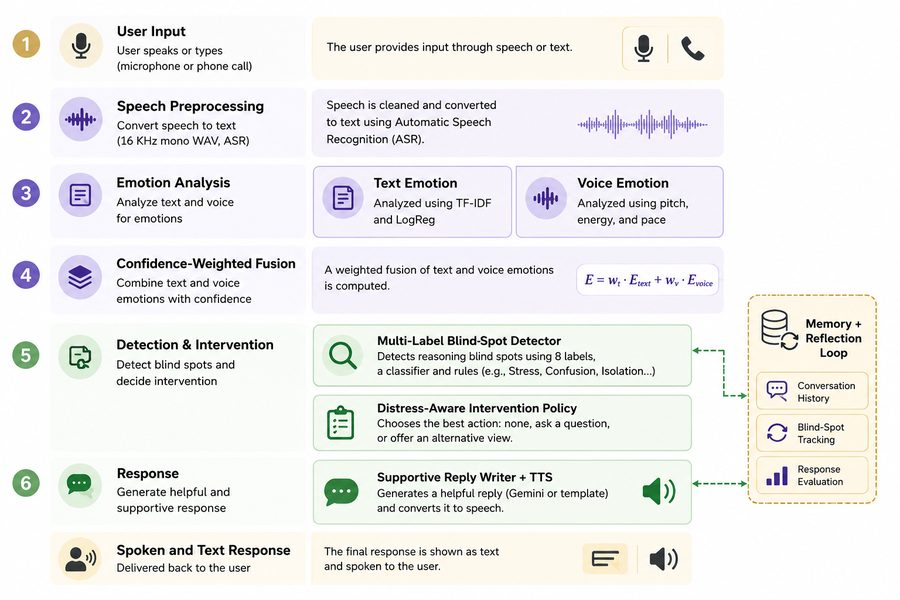
\includegraphics[width=\columnwidth]{fig1.png}}
\caption{Proposed six-stage system architecture.}
\label{fig:arch}
\end{figure}

The prototype used in this review differs a bit from the target architecture. It consists of a small Python server (only the standard library is used for the web component) together with a single-page browser interface. The browser records up to 15 seconds of audio input using the microphone, then converts it into 16~kHz mono WAV format and extracts meaningful audio features such as pitch, energy, and speech rate. The server performs emotion fusion, blind-spot detection, intervention decision making, and memory retrieval. If there is a Gemini API key, Gemini is used for transcription and validation as well as for producing the final reply; otherwise, templated replies are used. The telephony layer is not implemented, which means that user interaction takes place through the browser instead of the telephone.

%=====================================================================
\section{Data Sources and Representation}
The experiment is conducted using four types of data (refer to Table~\ref{tab:data}).

The first type is composed of GoEmotions \cite{r24} -- a Reddit-based corpus that has emotion labels for 27 emotion categories -- and MELD \cite{r25}, which contains dialogue sentences from a TV series with emotion labels. One of the teammates downloads text and label files and aligns their labels with our five-category scheme (stressed, sad, frustrated, happy, neutral). MELD's audio files were not downloaded due to their large volume, and therefore training of the speech model was not conducted on MELD.
The second type of data includes our own blind-spot corpus, gathered since no public dataset applicable to this experiment could be found. This corpus consists of 614 rows after duplicate removal: 53 rows manually written with single emotion labels, 60 with several emotion labels, and 501 generated with the help of templates (461 single-label and 40 multi-label). Out of these, 140 rows show absence of blind spots, providing an opportunity for the model to learn sound reasoning. An earlier version of our generator used the LIAR \cite{r26} dataset to generate weak labels, but this was stopped because false statements do not necessarily mean reasoning errors, and the model would otherwise learn keyword-based rules only.
The third type is a relatively small corpus of 458 sentences representing a small emotion lexicon, mostly template-generated and complemented by hand-crafted seeds.
The fourth type is represented by 150 real patients' questions collected from the therapist question-and-answer Kaggle dataset. This data is unlabeled and manually annotated by a single annotator as a test set. Inter-annotator agreement assessment was not carried out.

\begin{table}[htbp]
\caption{Data Used in the Project}
\label{tab:data}
\begin{center}
\small
\begin{tabular}{|p{1.6cm}|p{2.0cm}|p{3.4cm}|}
\hline
\textbf{Dataset} & \textbf{Size} & \textbf{Used for} \\
\hline
GoEmotions \cite{r24} & 43,410 / 5,426 / 5,427 (train/dev/test) & Text emotion (research scripts, prototype tests) \\
\hline
MELD text \cite{r25} & 9,990 / 1,110 / 2,611 & Text emotion; speech audio not downloaded \\
\hline
Blind-spot set (ours) & 614 rows, 8 labels, 140 with none & Train blind-spot classifier \\
\hline
Emotion set (ours) & 458 rows, 5 classes & Train text emotion model \\
\hline
Synthetic conversations & 120 train / 30 eval conversations & Test memory and reasoning stages \\
\hline
Real questions (Kaggle) & 150, hand-labelled by one person & Real-text test of the baseline \\
\hline
\end{tabular}
\end{center}
\end{table}

%=====================================================================
\section{Implementation Technologies}
The prototype implementation only needs Python 3.10 or its newer version along with the packages scikit-learn \cite{r30} and NumPy. The server uses the standard HTTP server from the standard library, while the user interface includes plain HTML and JavaScript with usage of the Web Audio API for both recording and pitch estimation. The more complex research scripts require PyTorch and Hugging Face Transformers. Table~\ref{tab:stack} describes the software stack divided into layers; the stack was assembled by analyzing the import statements in all code files, since there was no single requirements file for the project.

VADER \cite{r27} lexicon-based sentiment classifier is used as a baseline by two module versions. The embeddings of Sentence-BERT \cite{r28} with FAISS index \cite{r29} are used by one memory module.

\begin{table}[htbp]
\caption{Software Stack by Layer}
\label{tab:stack}
\begin{center}
\small
\begin{tabular}{|p{2.0cm}|p{5.0cm}|}
\hline
\textbf{Layer} & \textbf{Tools} \\
\hline
Web interface & HTML, JavaScript, Web Audio API, browser SpeechRecognition \\
\hline
Server & Python 3.10+, http.server, json, urllib \\
\hline
Classical ML & scikit-learn (TF-IDF, logistic regression), NumPy, joblib \\
\hline
Deep learning (research scripts) & PyTorch, torchaudio, Transformers, datasets, accelerate, sentencepiece \\
\hline
Audio & librosa, soundfile, sounddevice, simpleaudio \\
\hline
Memory / sentiment & FAISS, sentence-transformers, vaderSentiment \\
\hline
LLM and speech & Google Gemini (gemini-2.5-flash, Gemini TTS) via REST and google-genai \\
\hline
Utilities & pandas, SciPy, matplotlib, tqdm, python-dotenv \\
\hline
\end{tabular}
\end{center}
\end{table}

%=====================================================================
\section{Methodology}
The following section details the pipeline on a stage-by-stage basis and specifies the thresholds used in the codebase.

\subsection{Speech Input}
The browser records the user for a maximum of 15 seconds. The recording is transformed to mono 16~kHz 16-bit WAV format and clipped to keep the last 20 seconds of audio. In cases where the browser cannot decode the recorded audio format, raw samples returned via the Web Audio API are used. The server limits the file size to 12~MB for audio files. Transcripts are generated from the browser's speech recognizer, Gemini, or user input and are modifiable.

\subsection{Text and Voice Emotion}
Text-based emotion detection uses a TF-IDF model of word n-grams (1--2) and character n-grams (3--5) followed by logistic regression with balanced class weights. A short keyword rule serves as a back-off strategy in order to avoid losing explicitly stated emotions (e.g., ``overwhelmed'') in case of neutral model classification.

As far as vocal emotion is concerned, the browser estimates the pitch of each 46~ms chunk of audio using autocorrelation in the 70--350~Hz range. Then the server maps median pitch, pitch variability, mean energy, and words-per-minute into a categorical label via simple heuristic rules. For example, high energy with considerable pitch variability and fast talking means stress, while low energy with low pitch means sadness. This heuristic is not a model, and the confidence values (in the range of 0.52--0.67) were assigned manually.

\subsection{Fusion}
The two emotion estimates are fused using a confidence-weighted rule (Algorithm~\ref{alg:fuse}). Confidence of text-based emotion estimation is limited by 0.35. When modalities agree, the process is straightforward. If the text signal is neutral and the voice signal is one of stress, sadness, or frustration, the result based on voice is chosen, as lexical information can sometimes hide true emotions. In any other case, the voice signal dominates only when its confidence is higher than that of the text signal by more than 0.12. The weights are computed as ratios of respective confidences normalized by their sum, and these weights are displayed in the interface.

\subsection{Blind-Spot Detection}
This detection algorithm includes two components integrated into the workflow. The first component applies a one-vs-rest logistic regression on the same TF-IDF features, predicting the probability of all eight classes for the given instance. Labels are selected only when their probability is 0.42 or more, with at most four labels possible per message.

The second component represents a rules layer, implemented through regular expressions for overgeneralization detection and indicators of logical leap (keywords ``always'' or ``never,'' and connectors such as ``so,'' ``therefore,'' and ``that means''). For logical leap labels, the rules layer additionally splits the detected sentence into a premise and conclusion, with extra weight assigned to very thin premises (``my friend,'' ``once'') and very certain conclusions (``definitely''). If the label is found by both components, then the label with the highest confidence is taken. The proposed cues are not accusations but rather clues, and the interface explicitly states this.

With the configurations of Gemini, there is a secondary invocation that considers the transcript, classifier output, intervention decision, Gemini's memory, and the user's reaction to the last question asked. It may either suppress any detected blind spot lacking transcript support or introduce a blind spot that was previously unnoticed. This step was added since the trained classifier is not reliable enough (see Section~\ref{sec:results}).

\subsection{Adaptive Intervention}
The key parameter for the action of the companion is the highest blind-spot confidence (Algorithm~\ref{alg:decide}). Below the confidence level of 0.45, there is only an acknowledgement of the user, without further questions. Levels between 0.45 and 0.75 trigger a single reflection question. Above 0.75, the intervention includes an alternative, gentler reading of the user's statement, followed by a question. If the user shows sadness, stress, or frustration, then the strongest variant is always reformulated as a question, to show that the companion is sympathetic.

\subsection{Response, Memory, and Reflection Loop}
In Gemini, the reply is generated with a prompt that defines the tone (warm and nonjudgmental), absence of diagnostic labeling, maximum length of 70 words, and plain language for oral speech. Without Gemini, the template chooses the opening phrase depending on the detected emotion and adds the corresponding question for the detected blind spot. The reply can be delivered through the text-to-speech module of Gemini or the web browser interface.

In the demonstrated version of Gemini, memory is kept in RAM and represents the history of conversation containing previous turns in text form. Jaccard similarity (word overlap) between the new message and each stored turn is computed; if it is larger than 0.12, then the turn is used to generate the reply. For the reflection loop, the next user reply is checked for reconsideration words like ``maybe,'' ``you're right,'' or ``good point,'' and resistance words like ``whatever'' or ``stop.''

%=====================================================================
\section{Algorithms and Pseudocode}
This subsection discusses the two algorithms behind the system: Fusion Rule and Intervention Policy. Both are deliberately made concise and clear, so that everybody can easily see why the system acted in a particular way.

\subsection{Algorithm 1: Fusion Rule}
Algorithm~\ref{alg:fuse} combines emotion signals from text and speech. It ensures that neither modality has an unfair advantage and sets confidence levels as criteria for choosing the emotion label. The algorithm also calculates the weights of text and speech inputs, making the decision process interpretable.

\begin{algorithm}[htbp]
\caption{$\textsc{Fuse}(t_e, t_c, s_e, s_c)$}
\label{alg:fuse}
\begin{algorithmic}[1]
\State $t_w \leftarrow \max(0.35,\, t_c)$
\If{$t_e = s_e$}
    \State $label \leftarrow t_e$
\ElsIf{$t_e = \text{neutral}$ \textbf{and} $s_e \in \{\text{stressed, sad, frustrated}\}$}
    \State $label \leftarrow s_e$
\ElsIf{$s_c > t_w + 0.12$}
    \State $label \leftarrow s_e$
\Else
    \State $label \leftarrow t_e$
\EndIf
\State $w_{text} \leftarrow t_w/(t_w + s_c)$
\State $w_{speech} \leftarrow s_c/(t_w + s_c)$
\State \Return $label, (w_{text}, w_{speech})$
\end{algorithmic}
\end{algorithm}

\subsection{Algorithm 2: Intervention Policy}
Algorithm~\ref{alg:decide} defines the reaction to detected blind spots. It is based on the confidence level of the strongest finding and decides whether the companion should stay silent, ask a reflective question, or provide an alternative perspective. However, if the user is already sad, stressed, or frustrated, the algorithm is more conservative about interventions and formulates them in the form of a question.

\begin{algorithm}[htbp]
\caption{$\textsc{Decide}(findings, emotion)$}
\label{alg:decide}
\begin{algorithmic}[1]
\If{$findings$ is empty}
    \State \Return NONE
\EndIf
\State $top \leftarrow$ finding with highest confidence $c$
\If{$c < 0.45$}
    \State $type \leftarrow$ NONE
\ElsIf{$c < 0.75$}
    \State $type \leftarrow$ QUESTION
\Else
    \State $type \leftarrow$ ALTERNATIVE
\EndIf
\If{$type = $ ALTERNATIVE \textbf{and} $emotion \in \{\text{sad, stressed, frustrated}\}$}
    \State $type \leftarrow$ QUESTION \Comment{soften response}
\EndIf
\State \Return $(type, top.label)$
\end{algorithmic}
\end{algorithm}

\subsection{Blind-Spot Union Step}
Moreover, the step of finding the union of the blind spots combines the classifier labels with those detected via rules. The labels are retained only if they are above the threshold of probability, and the four most confident are selected. In future versions, the transformer-based classifier (DeBERTa-v3 with sigmoid outputs) will enable per-label thresholds, which our training scripts currently support but have not yet been used.

%=====================================================================
\section{Results and Discussion}
\label{sec:results}

\subsection{What the Prototype Does}
The prototype receives either a recording or a typed text and produces the transcript, text emotion, voice estimate, fused emotion with weights, detected blind spots with an explanation and a question, the decision about the intervention, the retrieved memories, and the reply. It can vocalize the reply and reset its memory. We wrote 19 unit tests that cover the main path, cue detection, memory, invalid input, audio payload checks, a mocked Gemini flow, and the HTTP endpoints, and they all pass.

We also tried a demo sequence. For example, the sentence ``My friend did it and it worked out for him, so it will definitely work for me'' is detected as a logical leap and triggers a question asking what else would need to be true.

\subsection{Measured Results}
Table~\ref{tab:results} and Fig.~\ref{fig:f1} show the measured performance. This is significant since performance differs greatly between examples with some doing extremely well while others do extremely badly, and therefore finding out the reasons for the difference is crucial.

Text Emotion model reached an accuracy of 63.7\% and macro-F1 of 0.638. Yet, considering the fact that the test set was created from the same templates as the training set, the performance is highly overoptimistic. More conservative estimation done by a teammate using a simpler VADER- and keyword-based method resulted in about 58\% accuracy on 300 GoEmotions examples and 54\% accuracy on 300 MELD examples, which are definitely more realistic benchmarks.

As for the blind spots, the six-label baseline received a perfect score on test sentences created from identical templates and scored almost as good on sentences about new topics. This is due to the fact that the label is determined by the wording and not the topic. With new wording, macro-F1 falls to 0.291, and even lower to 0.125 on real patient questions. The model used in the application, which was trained only on synthetic rows, reached micro-F1 of 0.378 on 113 handwritten rows. In other words, the model learns templates but does not have any reasoning abilities. This core flaw explains the necessity to use Gemini as the detector of detections and also the reserved attitude towards the accuracy claims.

\begin{table}[htbp]
\caption{Measured Results of the Text Models}
\label{tab:results}
\begin{center}
\small
\begin{tabular}{|l|c|c|}
\hline
\textbf{Model / Test Set} & \textbf{Micro-F1} & \textbf{Macro-F1} \\
\hline
Text emotion, 5 classes & 0.924 & 0.926 \\
Blind spots, 8 labels (app) & 0.378 & 0.291 \\
Blind spots, 6 labels (baseline) & 1.000 & 1.000 \\
Unseen wording & 0.665 & 0.660 \\
Unseen topics & 0.991 & 0.992 \\
LIAR, weak labels & 0.531 & 0.470 \\
Real questions & 0.181 & 0.125 \\
\hline
\end{tabular}
\end{center}
\end{table}

\begin{figure}[htbp]
\centerline{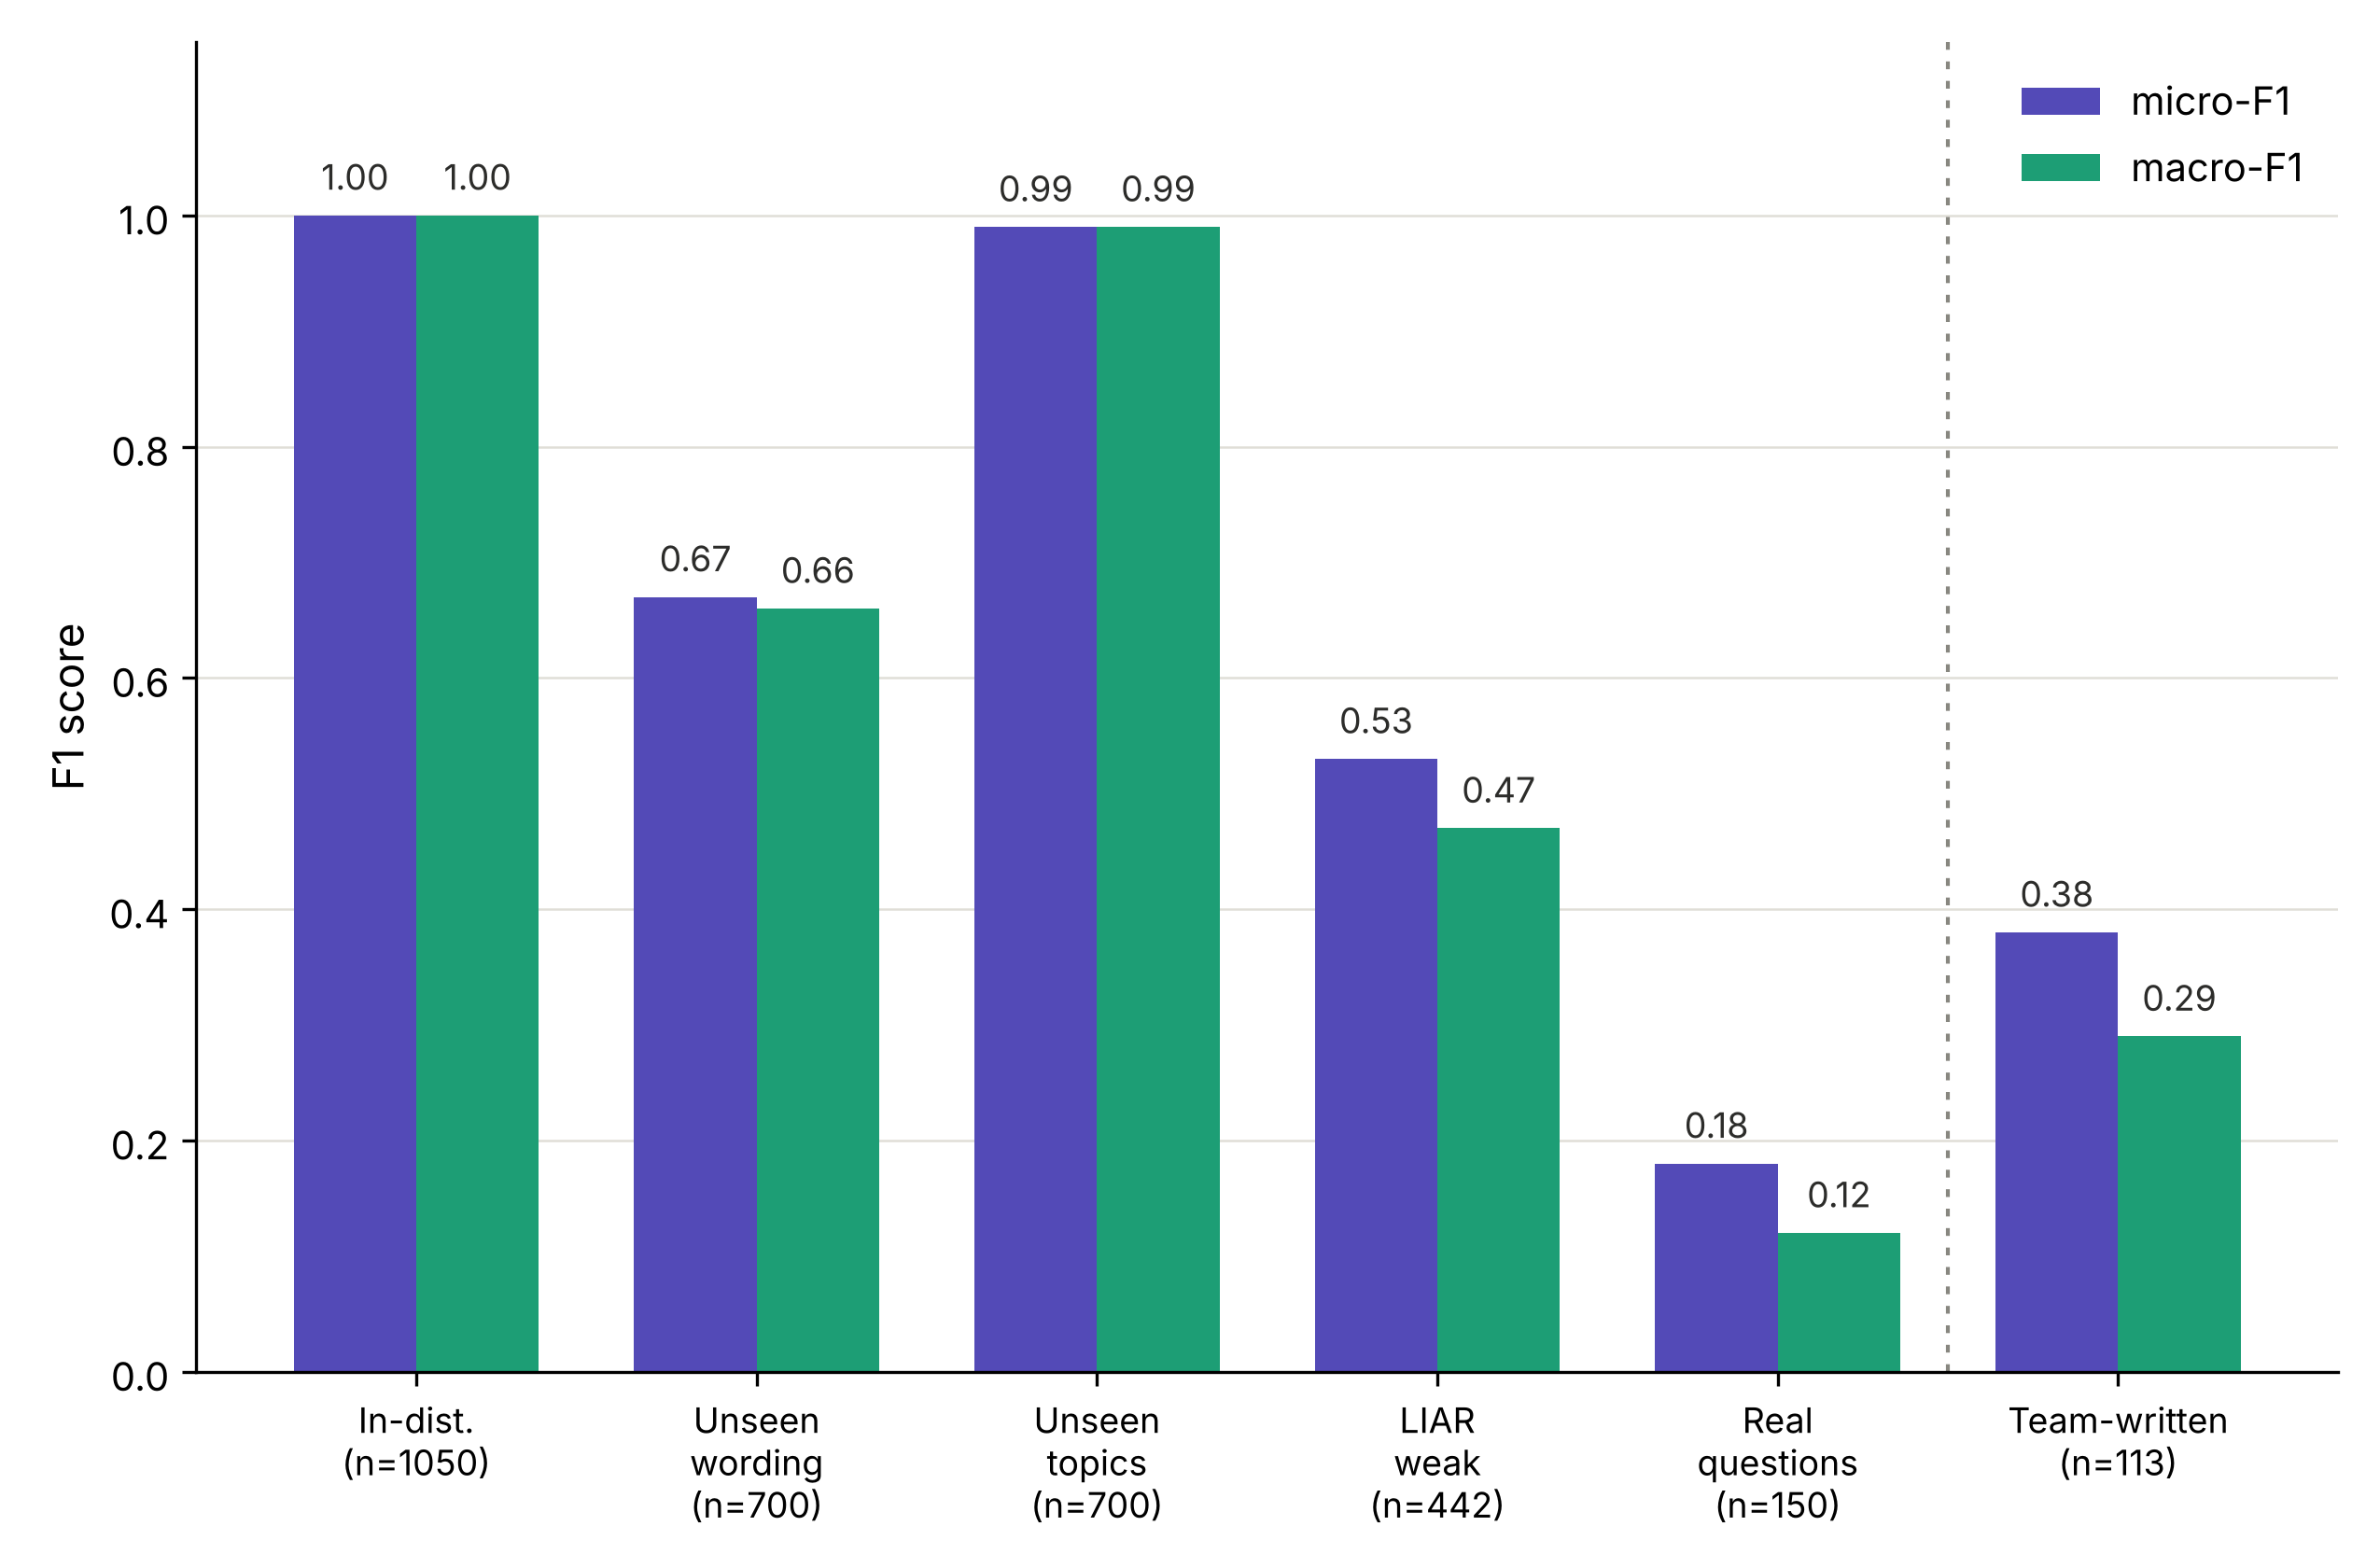
\includegraphics[width=\columnwidth]{fig2.png}}
\caption{Micro-F1 and Macro-F1 scores across different test sets.}
\label{fig:f1}
\end{figure}

\subsection{Limitations}
\textbf{Data.} Most training rows are generated from templates, so the labels reflect our generator's intentions rather than real conversations. There is no inter-annotator agreement. Real speech is noisier, with filler words, incomplete sentences, and missing punctuation.

\textbf{Voice emotion.} The voice estimate uses manually set thresholds on pitch, energy, and pace. It was never tested on labeled speech and may misbehave for different voices, microphones, or room conditions. The Gemini voice estimate is also unvalidated. Although Wav2Vec2 and WavLM scripts exist, they were not trained due to lack of audio data.

\textbf{Untrained deep models.} The RoBERTa, WavLM, DeBERTa-v3, and attention fusion code is written and syntactically checked, but not trained or evaluated in this snapshot. Module versions created by different teammates use different label sets (five classes in some, seven MELD classes in others), which should be unified.

\textbf{Missing features.} The phone-call interface, real-time streaming, and latency measurement are not implemented. Humour is also missing. The current prompt enforces a warm and non-judgmental tone but has no humour instruction, and tone checking is only prompt-level. Memory is lost once the server stops, and the system works only in English.

\textbf{Privacy and safety.} With Gemini enabled, recordings and transcripts are sent to Google. Users may share private information, so explicit consent is required. This system is not a therapist and should not be used in crisis situations. We have not tested its response to self-harm statements, and a safe hand-off to a human or helpline must be added before deployment.

\subsection{Planned Evaluation}
We plan three studies. First, to collect 200--500 role-played or real call transcripts, annotate them with two annotators, report agreement, and use them as a test set. Second, to train DeBERTa-v3 and RoBERTa on a larger dataset and compare them with the TF-IDF baseline on the same held-out wording split. Third, to fine-tune a speech emotion model on labeled audio and test whether fusion outperforms text alone, which our prototype has not yet demonstrated. Finally, we will measure latency (time from end of user speech to start of reply) and conduct a small user study on helpfulness, warmth, and non-judgmentality of replies.

%=====================================================================
\section{Conclusion and Future Scope}
EchoMind is a voice-enabled companion which recognizes reasoning blind spots and responds tactfully. We have designed the system with an integrated prototype that involves text and voice emotion, a fusion rule, eight-label blind-spot detection, a confidence-based intervention policy, a memory element, and a reflection loop. The system works and satisfies the test cases, but it appears that models trained on synthetic data are not transferrable to actual text input. Therefore, we use Gemini to validate the blind spots detected and do not claim accuracy for the overall system.

For future research, we plan to train transformers on real-life annotated data, remove the voice heuristic using a speech emotion model, design the phone-call interface with streaming support, add humour and tone checking, save memory with user consent, support regional Indian languages, and implement safe response strategies in case of emergencies. Once these improvements are made, a user study can be conducted to evaluate whether users find the feedback helpful, warm, and non-judgmental.

%=====================================================================
\begin{thebibliography}{00}
\bibitem{r1} A. T. Beck, \textit{Cognitive Therapy and the Emotional Disorders}. New York, NY, USA: International Universities Press, 1976.
\bibitem{r2} ``PECER: Empathetic response generation via dynamic personality extraction and contextual emotional reasoning,'' 2024.
\bibitem{r3} ``A joint model with contextual and speaker information for conversational causal emotion entailment,'' 2024.
\bibitem{r4} ``Empathetic response generation via regularized Q-learning,'' 2025.
\bibitem{r5} ``CACKS: Context-adaptive commonsense knowledge selection for empathetic dialogue generation,'' 2025.
\bibitem{r6} ``SURE: Synergistic uncertainty-aware reasoning for multimodal emotion recognition in conversations,'' 2026.
\bibitem{r7} ``Emotional support with conversational AI: Talking to machines about life,'' 2026.
\bibitem{r8} ``Longitudinal study on social and emotional use of AI conversational agent,'' 2025.
\bibitem{r9} ``Voice interaction with conversational AI could facilitate thoughtful reflection and substantive revision in writing,'' 2025.
\bibitem{r10} ``User interaction patterns and breakdowns in conversing with LLM-powered voice assistants,'' 2025.
\bibitem{r11} ``Voice assistants for mental health services: Designing dialogues with homebound older adults,'' 2024.
\bibitem{r12} ``Reflecti-Mate: A conversational agent for adaptive decision-making support through System 1 and System 2 thinking,'' 2026.
\bibitem{r13} A. D\'efossez \textit{et al.}, ``Moshi: a speech-text foundation model for real-time dialogue,'' arXiv:2410.00037, 2024.
\bibitem{r14} ``A high-speed, multimodal architecture for real-time contextual voice assistance,'' 2025.
\bibitem{r15} ``HumorGen: Cognitive synergy for humor generation in large language models via persona-based distillation,'' 2026.
\bibitem{r16} ``Perception of empathy in mental health care through voice-based conversational agent prototypes: Experimental study,'' 2025.
\bibitem{r17} ``Know your mistakes: Towards preventing overreliance on task-oriented conversational AI through accountability modeling,'' 2025.
\bibitem{r18} A. Radford \textit{et al.}, ``Robust speech recognition via large-scale weak supervision,'' arXiv:2212.04356, 2022.
\bibitem{r19} A. Baevski, H. Zhou, A. Mohamed, and M. Auli, ``wav2vec 2.0: A framework for self-supervised learning of speech representations,'' in \textit{Proc. NeurIPS}, 2020.
\bibitem{r20} S. Chen \textit{et al.}, ``WavLM: Large-scale self-supervised pre-training for full stack speech processing,'' \textit{IEEE J. Sel. Topics Signal Process.}, vol. 16, no. 6, pp. 1505--1518, 2022.
\bibitem{r21} Y. Liu \textit{et al.}, ``RoBERTa: A robustly optimized BERT pretraining approach,'' arXiv:1907.11692, 2019.
\bibitem{r22} P. He, J. Gao, and W. Chen, ``DeBERTaV3: Improving DeBERTa using ELECTRA-style pre-training with gradient-disentangled embedding sharing,'' arXiv:2111.09543, 2021.
\bibitem{r23} Gemini Team, Google, ``Gemini: A family of highly capable multimodal models,'' arXiv:2312.11805, 2023.
\bibitem{r24} D. Demszky \textit{et al.}, ``GoEmotions: A dataset of fine-grained emotions,'' in \textit{Proc. ACL}, 2020, pp. 4040--4054.
\bibitem{r25} S. Poria \textit{et al.}, ``MELD: A multimodal multi-party dataset for emotion recognition in conversations,'' in \textit{Proc. ACL}, 2019, pp. 527--536.
\bibitem{r26} W. Y. Wang, ```Liar, liar pants on fire': A new benchmark dataset for fake news detection,'' in \textit{Proc. ACL}, 2017, pp. 422--426.
\bibitem{r27} C. J. Hutto and E. Gilbert, ``VADER: A parsimonious rule-based model for sentiment analysis of social media text,'' in \textit{Proc. ICWSM}, 2014.
\bibitem{r28} N. Reimers and I. Gurevych, ``Sentence-BERT: Sentence embeddings using Siamese BERT-networks,'' in \textit{Proc. EMNLP-IJCNLP}, 2019, pp. 3982--3992.
\bibitem{r29} J. Johnson, M. Douze, and H. J\'egou, ``Billion-scale similarity search with GPUs,'' \textit{IEEE Trans. Big Data}, vol. 7, no. 3, pp. 535--547, 2021.
\bibitem{r30} F. Pedregosa \textit{et al.}, ``Scikit-learn: Machine learning in Python,'' \textit{J. Mach. Learn. Res.}, vol. 12, pp. 2825--2830, 2011.
\end{thebibliography}

\end{document}